\section{Cơ sở lý thuyết}
\subsection{Phát triển trò chơi}
\hspace*{0.5cm} \textit{Video game (hay trò chơi điện tử)} là trò chơi được vận hành bằng các thiết bị điện tử để tạo môi trường tương tác. Trải qua các giai đoạn lịch sử, với sự phổ biến và phát triển của công nghệ, trò chơi điện tử ngày càng phổ biến với người dùng hơn. Các máy, hay còn gọi là “nền tảng,” mà trên đó trò chơi điện tử được chơi có thể là máy tính cá nhân, máy game arcade (game thùng), máy chơi game kết nối với tivi gia đình, máy chơi game cầm tay, thiết bị di động như điện thoại di động, máy tính bảng,... với đủ mọi thể loại như casual, giải đố, các game double A hoặc triple A,...\\
\hspace*{0.5cm} \textit{Phát triển trò chơi điện tử} là một  quá trình sáng tạo, kết hợp các yếu tố nghệ thuật như thiết kế, đồ hoạ, âm thanh, hình ảnh và các yếu tố kỹ thuật như cấu trúc dữ liệu, xử lý đầu vào, thuật toán, AI,... để tạo ra một trò chơi điện tử. Quá trình này trải qua nhiều công đoạn khác nhau:\\
\begin{itemize}
	\item \textbf{Lên kế hoạch}: Nghiên cứu thị trường, xác định thể loại và concept chỉnh của trò chơi, mục đích và lên kế hoạch cho các cột mốc cho dự án.
	\item \textbf{Tiền sản xuất}: Khi ý tưởng đã được hình thành và kế hoạch đã được vạch ra rạch ròi thì giai đoạn này là giai đoạn dành cho việc thiết kế và hình thành nên cơ chế và thế giới game về mặt ý tưởng. Đây là bước rất quan trọng, có thể ảnh hưởng trải nghiệm chơi game về sau.
	\item \textbf{Sản xuất}: Đây là phần quan trọng nhất của quá trình, là quá trình tốn rất nhiều thời gian để thực sự tạo ra trò chơi điện tử theo từng thành phần phần và kết hợp chúng lại với nhau. Bước này cũng có thể là phần khó khăn nhất vì có thể phát sinh các vấn đề cần được giải quyết, trong khi một số yếu tố của trò chơi có thể phải bị cắt bỏ hoặc thay đổi. Điều này có thể kéo dài một vài tuần hoặc tháng cho thời gian phát triển.
	\item \textbf{Kiểm thử}: Khi phiên bản đầu tiên của trò chơi đã được sản xuất. Trò chơi phải được kiểm tra kỹ lưỡng để phát hiện bất kỳ vấn đề nào trong thiết kế trò chơi hoặc code có thể khiến trò chơi không hoạt động đúng cách. Debug giúp phát hiện và sữa chữa sự cố trong mã nguồn trò chơi. Nó cũng có thể làm phát sinh các vấn đề lớn hơn khi thiết kế trò chơi không hoạt động như dự kiến – ví dụ, một người chơi có thể phá vỡ trò chơi bằng cách tiếp cận các khu vực không được phép một cách không đúng.Kiểm tra không chỉ để tìm các vấn đề cụ thể. Nó cũng có thể đánh giá cảm giác tổng thể của trò chơi. Ví dụ, trò chơi có quá dễ hay quá khó không? Câu chuyện có lôi cuốn không? Kiểm tra có thể giúp trả lời những câu hỏi này.
	\item \textbf{Tiền phát hành}: Đến thời điểm này, trò chơi đã được phát triển thành một sản phẩm gần như sẵn sàng để phát hành. Một phiên bản beta của trò chơi có thể được gửi cho một số ít người chơi được chọn để nhận phản hồi và giúp xác định những thay đổi vào phút chót.Thời gian trước khi ra mắt cũng là lúc thực hiện các hoạt động marketing và quảng cáo thông qua trailer và áp phích, và các studio AAA sẽ trình bày một cách thu hút tại các hội chợ trò chơi. Phiên bản sớm của trò chơi có thể được gửi đến các nhà phê bình tại các tạp chí trò chơi và những chuyên gia khác, những người sẽ chơi trò chơi và đánh giá, sau đó được công bố trực tuyến.Các bài đánh giá có thể giúp tạo sự hứng thú nếu trò chơi được đánh giá cao, nhưng không đảm bảo sẽ phù hợp với quan điểm của cộng đồng game thủ rộng lớn. Có một số trường hợp trò chơi bị các chuyên gia cho điểm thấp nhưng cộng đồng game thủ lại đánh giá cao.
	\item \textbf{Phát hành}: Giai đoạn ra mắt bao gồm việc sửa các lỗi còn sót lại trong trò chơi để đảm bảo trò chơi sẵn sàng cho việc phát hành rộng rãi. Một số cải tiến nhỏ cũng có thể được thêm vào để hoàn thiện sản phẩm cuối cùng.
	\item \textbf{Hậu phát hành}: Sau khi phát hành, có thể xuất hiện các lỗi. Việc sửa lỗi là điều không thể tránh khỏi khi số lượng người chơi trò chơi (hy vọng) sẽ gặp phải các vấn đề. Việc sửa chữa các lỗi này càng sớm càng tốt thông qua các bản cập nhật là điều cực kỳ quan trọng để đảm bảo khách hàng có thể tận hưởng trò chơi và tạo ảnh hưởng tốt trong cộng đồng. Ngoài ra, trong giai đoạn hậu ra mắt, công việc vẫn có thể tiếp tục để tạo thêm nội dung cho trò chơi nhằm giữ chân người chơi. Nội dung bổ sung này thường được phát hành dưới dạng các bản cập nhật lớn theo mùa hoặc DLC (Downloadable Content - nội dung có thể tải xuống) đóng vai trò như một phần mở rộng cho game gốc. Quá trình phát triển nội dung mới có thể làm giai đoạn phát triển quay trở lại giai đoạn lên kế hoạch (cho các nội dung mới).
\end{itemize}
\subsection{Thiết kế màn chơi}
\hspace*{0.5cm} Một màn chơi là không gian những gì cốt lõi diễn ra trong game. Nơi này đặt ra những giới hạn cho người chơi trong việc tương tác với game. Có sự đa dạng trong từng level. Mỗi level có thể có một số điểm tương đồng, nhưng mỗi màn sẽ có những nét đặc trưng khác nhau.\\
\hspace*{0.5cm} Thiết kế màn chơi là một giai đoạn của quá trình phát triển trò chơi nơi các nhà phát triển tập trung tạo ra các không gian này, bao gồm các cấp độ, bản đồ và nhiệm vụ trong game. Việc thiết kế trò chơi là việc kết hợp các yếu tố cấu thành nên trải nghiệm người chơi, bao gồm cơ chế game, gameplay, cốt truyện,...\\
\hspace*{0.5cm} Tuy nhiên, việc thiết kế màn chơi không phải để cho có. Việc thiết kế màn chơi cần có một mục đích nào đó, ví dụ như kể chuyện, có nhân vật và phục vụ cho mục đích rõ ràng trong game. Hơn hết, người thiết kế phải tập trung vào trải nghiệm người chơi, hơn là cảm nhận bản thân. Và màn chơi phải thực sự cuốn hút và vui để mang đến trải nghiệm cho người chơi\\
\hspace*{0.5cm} Mục tiêu của việc thiết kế màn chơi là tạo ra các sự kiện tương tác trong môi trường game sao cho chúng mang tính thử thách người chơi. Giúp người chơi đạt được cảm giác vui sướng khi hoàn thành và có mong muốn tiếp tục gắn bó với game.\\
\subsubsection{Các bước thiết kế một màn chơi}
\hspace*{0.5cm} Để thiết kế màn chơi, cần tập trung vào các bước chính sau:
\begin{enumerate}
	\item \textbf{Xác định lại giới hạn dự án}\\
	Các ý tưởng có thể có rất nhiều, trông chúng có thể rất hay nhưng mà ta cũng nên nhìn lại xem giới hạn của dự án có phù hợp cho ý tưởng này không, từ đó chọn được các ý tưởng phù hợp. Nó có thể đến từ bản chất của dự án hoặc kỹ thuật. Người thiết kế màn chơi cần hiểu rõ các giới hạn này để thiết kế màn chơi sao cho hợp lý.\\
	\hspace*{0.5cm} Về bản chất của dự án. Điều cần phải chú ý nhất là người chơi cũng như nền tảng hiện thực. Ta cần xác định đối tượng người chơi chủ đạo của game (là trẻ em, người trưởng thành hay người cao tuổi, là nam hay nữ, có phải là mẹ bỉm sữa hay không,...) cũng như nền tảng để chơi (mobile, PC hay console). Điều này ảnh hưởng đến thời gian hoàn thiện, độ dài và độ khó của màn chơi cũng như phong cách đồ hoạ. Những dự án làm trên mobile sẽ nhanh hơn so với PC hay console. Những trò chơi nhắm đến đối tượng trẻ em thì độ dài màn chơi sẽ ngắn, độ khó cũng dễ hơn cũng như phong cách đồ hoạ cũng sẽ nhẹ đô hơn so với các game dành cho lứa tuổi người trưởng thành. Ta không thể sản xuất một tựa game có phong cách đồ hoạ máu me, hoặc chủ đề có liên quan đến chiến tranh cho đối tượng là trẻ em được.\\
	\hspace*{0.5cm} Về vấn đề kỹ thuật, người thiết kế màn chơi phải giữ cho game có tính nhất quán về mặt công nghệ. Người thiết kế cần biết dự án sẽ sử dụng công nghệ nào, phong cách đồ hoạ ra sao, âm thanh, nhạc nền như thế nào. Một trò chơi không thể sử dụng lẫn lộn đồ hoạ pixel và đồ hoạ vector nếu không có mục đích cụ thể, hoặc có mục đích nhưng sử dụng không hợp lý. Một trò chơi về chiến tranh thế giới thời hiện đại không thể xuất hiện các yếu tố như pháp sư, phù thuỷ hay kiếm sĩ trong các tựa game RPG được. Ngược lại, một trò chơi RPG Fantasy nếu không có yếu tố liên quan đến thế giới thực thì không thể nào có thứ gọi là súng được. Ngoài ra  Ngoài ra, hiệu ứng ánh sáng và môi trường trong game cũng là một vấn đề đáng lưu tâm. Ở các tựa game kinh dị hù doạ hoặc truy đuổi, môi trường và ánh sáng sẽ tác động nhiều đến cảm xúc của người chơi, có thể tạo cho người chơi cảm giác hồi hộp, thót tim nếu sử dụng hợp lý.\\
	\hspace*{0.5cm} Dưới đây là một game có thiết kế màn chơi có vấn đè về kỹ thuật, trong việc sử dụng cả pixel art, vector art và hiệu ứng ánh sáng chưa hợp lý.\\
	\begin{figure}[H]
		\centering
		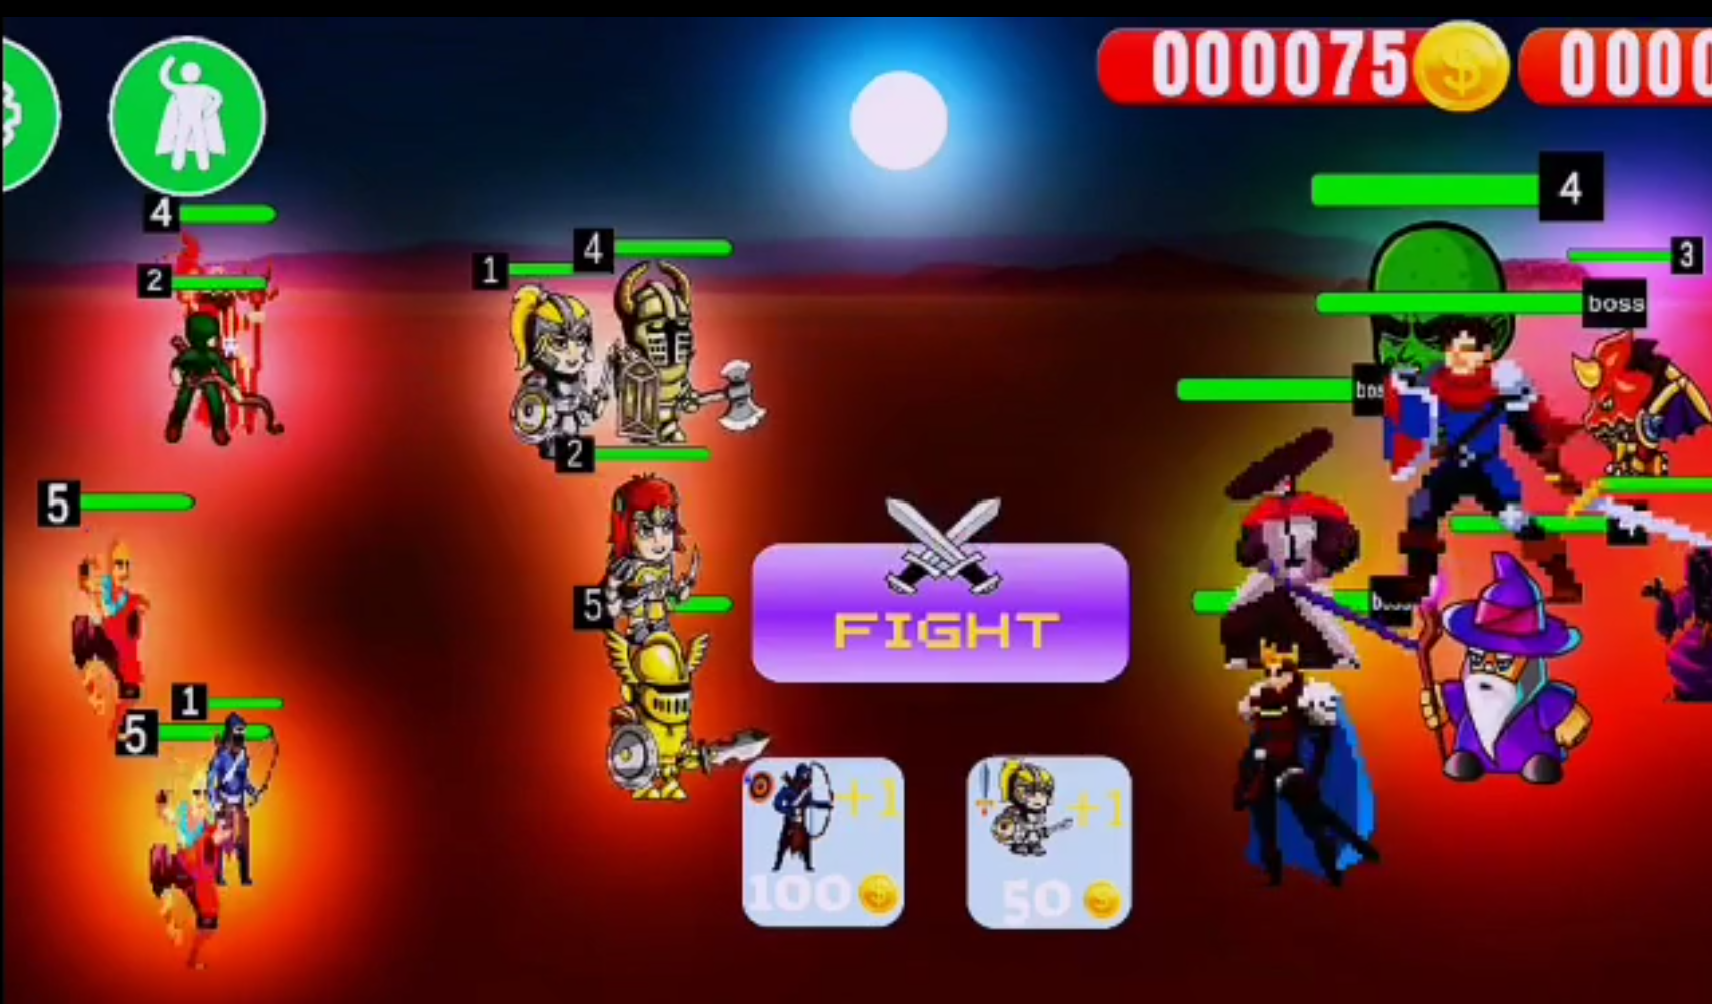
\includegraphics[width=\textwidth]{Images/AGameSuck.png}
		\vspace{0.5cm}
		\caption{Một màn chơi của game gặp vấn đề về kỹ thuật}
	\end{figure}

	\item \textbf{Lên ý tưởng và phác hoạ sơ bộ cấu trúc.}\\
	\hspace*{0.5cm}  Ở giai đoạn này, các thành viên khác trong dự án sẽ tiến hành lên ý tưởng và phác hoạ lên diẽn biến chính của cốt truyện cũng như xác định sơ bộ các thành phần khác của trò chơi như hình ảnh, âm thanh. Để việc thiết kế được dễ dàng hơn, người thiết kế có thể chia màn chơi thành các zone nhỏ sao cho dễ quản lý. Người thiết kế nên nghĩ đến màn chơi nếu chia thành nhiều zone sẽ ra sao và thiết kế từng zone riêng biệt để đạt hiệu suất cao và đơn giản hơn so với thiết kế toàn bộ màn chơi là một khối lớn.\\ 
	
	
	\item \textbf{Vẽ Bubble Diagram (lưu đồ Bong bóng).}\\
	\hspace*{0.5cm}  Trước khi bắt đầu đầu tư vào dự án, cần phải biết được tổng quan của các màn chơi sẽ như thế nào. việc giải thích bằng văn nếu không có sự hiệu quả sẽ gây khó hiểu cho người tiếp cận. Vì thế nên việc sử dụng lưu đồ sẽ phát huy tính hiệu quả, giúp cho người tiếp cận có cái nhìn tổng quan về màn chơi, bao gồm các zone chứa những gì và các zone được liên kết như thế nào. Ở giai đoạn này, sau khi phân chia màn chơi thành các vùng nhỏ và thiết kế chúng, người thiết kế sẽ kết nối các vùng đó với nhau thông qua một lưu đồ bong bóng.\\
	\textbf{Một số quy tắc khi vẽ lưu đồ:}
	\begin{itemize}
		\item Mỗi node trong đồ thị sẽ tượng trưng cho một zone của màn chơi.
		\item Mỗi node có thể kết nối với node khác bằng một và chỉ một mũi tên, đi từ ra từ node này đến node được chỉ định, một node có thể có thể có nhiều mũi tên chỉ ra, cũng như cũng có thể được nhiều mũi tên chỉ vào.
		\item Trên  mỗi mũi tên có thể có một ghi chú, có thể là điều kiện, ghi chú đường tắt,...
	\end{itemize}
	\begin{figure}[H]
		\centering
		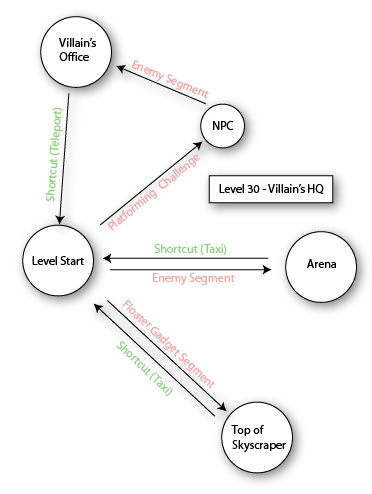
\includegraphics[width=7cm]{Images/bubblediagram.jpg}
		\vspace{0.5cm}
		\caption{Lưu đồ bong bóng}
	\end{figure}
	\hspace*{0.5cm} 
	\item \textbf{Tạo ra bản sơ lược của màn chơi}\\
	\hspace*{0.5cm}  Ở giai đoạn này, những nhà thiết kế màn chơi sẽ bắt đầu thiết kế một bản sơ lược cho màn chơi. Các bản thiết kế này có thể là thiết kế ở trên giấy, các phần mềm đồ hoạ như Adobe Illustrator hay
	trực tiếp trên các game engine như Unity, Unreal, ... Với mỗi node trong đồ thị tương ứng với một zone, một room, ta sẽ sắp xếp thứ mà người chơi sẽ phải gặp trong zone đó, đó có thể là quái vật, rương thưởng, hoặc quái vật giả rương thưởng, hoặc các câu đố đòi hỏi người chơi phải giải quyết được mới được tính là clear.  Ngoài ra, họ sẽ nghĩ đến phương pháp để kết nối các zone với nhau dựa theo mũi tên của đồ thị bong bóng cũng như điều kiện trên đó (nếu có).\\
	\hspace*{0.5cm} Để một màn chơi tổng thể hấp dẫn, dựa theo nhiều trò chơi khác đã thành công trên thị trường, mỗi zone liên tiếp nhau nên có độ khó tăng dần lên. Việc việc mỗi zone tăng dần độ khó như vậy sẽ luôn tạo cho người chơi các thách thức để họ vượt qua. Từ đó, trò chơi sẽ gia tăng trải nghiệm chơi game của người chơi.\\
	\hspace*{0.5cm} Nếu muốn di chuyển sang vùng kế tiếp thì phải clear vùng hiện tại. Ví dụ, phải clear được vùng 1 thì mới có thể đi đến vùng 2.  Vùng cuối cùng (hoặc điểm cuối cùng trên lưu đồ) sẽ là nơi được đặt một con quái vật boss hoặc mini-boss, nếu clear được thì sẽ được phần thưởng của màn chơi đó.\\
	\hspace*{0.5cm} Trong giai đoạn này, một vài thông số của màn chơi như diện tích, chiều cao, khoảng cách có thể chưa cố định. Người thiết kế và các lập trình viên sẽ kiểm thử và căn chỉnh dần cho phù hợp với ý đồ của nhà thiết kế.\\
	\item \textbf{Hoàn thành thiết kế màn chơi}\\
	\hspace*{0.5cm} Đây là giai đoạn cuối cùng, người thiết kế màn chơi sẽ hoàn thành màn chơi từ thiết kế sơ bộ ở giai đoạn 4.\\
	\hspace*{0.5cm} Người thiết kế màn chơi sẽ kết nối các vùng của màn chơi với nhau. Ở những vùng có thể di chuyển qua lại với nhau, đó có thể đơn giản chỉ là một cánh cổng hay đường hầm. Ở MeowSQL Knight, việc di chuyển 2 vùng khác nhau là tự nhiên, tuy nhiên để di chuyển cần phải clear zone hiện tại.\\
	\hspace*{0.5cm} Các zone phải được liên kết mới nhau sao cho phải với mỗi node có ít nhất một đường đi từ node bắt đầu, đi qua node hiện tại và đến node kết thúc. Nghĩa là không được có đường cùng trong màn chơi.\\
	\hspace*{0.5cm} Sau khi hoàn thành thiết lập toàn bộ bản đồ và kiểm thử, các thông số có thể thay đổi được ở giai đoạn 4 phải được thiết lập cố định lại.
\end{enumerate}
\subsubsection{Một số mẹo khi thiết kế màn chơi}
\hspace*{0.5cm}  Khi thiết kế một màn chơi, có một số mẹo chúng ta có thể tham khảo để kết quả đạt được tốt hơn.
\begin{itemize}
	\item \textbf{Thiết kế có mục đích rõ ràng: } Mỗi màn chơi phải có một mục đích tại sao nó lại tồn tại. Nó có thể là để người chơi học tập cách sử dụng một cơ chế nào đó của trò chơi và luyện tập các cơ chế đã học hoặc giúp cho cốt truyện được làm rõ và đưa đến người chơi. Ở một số trò chơi có cốt truyện, một vài màn chơi có đóng vai trò mở rộng cốt truyện ra.\\
	Từ các mục đích ban đầu, người thiết kế màn chơi phải luôn tập trung thiết kế để phục vụ mục đích đó. Tránh tập trung vào quá nhiều mục tiêu rời rạc, tránh làm level bị nhồi nhét quá nhiều. Điều này sẽ làm người chơi không bị choáng ngợp vì có quá nhiều thứ diễn ra trong màn chơi. Nếu vẫn muốn màn chơi có nhiều mục đích, hãy chắc chắn nó hợp với nhau và không làm cho màn chơi bị rối
	\item \textbf{Tập trung vào tính thực tế và sự đắm chìm khi chơi: } Tính thực tế cũng rất quan trọng và không nên xem nhẹ. Dù bối cảnh có là thế nào, viễn tưởng hoặc huyền ảo thế nào cũng nên thiết kế màn chơi sao cho người chơi cảm thấy vẫn có tính thực tế trong đó. Điển hình là trọng lực, dù cho nhân vật ở trong bất cứ thế giới game nào, thì cũng luôn bị trọng lực tác động vào. Ở các trò chơi bắn súng, người chơi thường thích việc nhà phát hành làm nó trông thực tế nhất có thể, bao gồm trọng lượng súng ảnh hưởng đến tốc độ di chuyển và độ giật khi bắn, độ giật của súng khác nhau, cũng như độ rơi của đạn khi bắn tầm xa. Trong các game về bóng đá, người chơi sẽ quan tâm đến logic trái bóng và cầu thủ trong các tình huống, về việc bắt lỗi và thẻ phạt của trọng tài, đặc biệt là các tình huống nguy hiểm trong vòng cấm.\\
	Nếu áp dụng các yếu tố thực tế một cách hợp lý, người chơi cảm nhận được sự thực tế trong trò chơi. Dần dần, họ bắt đầu chìm đắm vào trò chơi. Việc đắm chìm vô cùng quan trọng, nó cho thấy xu hướng yêu thích và sẽ gắn bó với nó lâu dài. Khi người chơi đã bắt đầu chìm đắm trong trò chơi, họ sẽ bắt đầu quan tâm đến các khía cạnh khác của trò chơi như cốt truyện, đồ hoạ, âm thanh,...
	\item \textbf{Một thử thách không quá dễ dàng nhưng không khó chịu: } Một màn chơi mang tính thử thách hoàn toàn khác với màn chơi khó đến mức gây khó chịu.\\
	Người chơi thích chơi game bởi vì tính thử thách của nó. Các thử thách này sẽ gây khó dễ cho người chơi, đòi hỏi sự rèn luyện, cùng với một khao khát mãnh liệt để vượt qua. Khi đã vượt qua được thử thách, một lượng dopamine được sinh ra khiến người chơi có cảm giác sảng khoái, khiến họ muốn tiếp tục vượt qua thử thách kế tiếp. Đây chính là mục đích cuối cùng mà các màn chơi muốn mang đến cho người chơi. Với dạng trò chơi mang tính chiến thuật như các game bóng đá, đôi khi trò chơi sẽ có một vài màn chơi khó, việc sử dụng một đội hình cố định có thể gặp khó khăn, đòi hỏi phải thay đổi chiến thuật như sử dụng cầu thủ khác, đổi sơ đồ đội hình sao cho qua được màn chơi. Người chơi sẽ cần thử nhiều loại đội hình. Đến một lúc nào đó, họ sẽ tìm ra một đội hình để vượt qua được màn chơi.\\
	Tuy nhiên, đôi khi những người thiết kế màn chơi không tránh khỏi việc trở thành một màn chơi gây khó chịu. Người thiết kế màn chơi đôi khi suy nghĩ rằng chỉ cần đưa hết tất cả những thứ khó nhất vào màn chơi sẽ làm màn chơi mang tính thách thức, hoặc họ nghĩ rằng họ có thể "bào tiền" từ người chơi thông qua các vật phẩm mua bằng tiền thật có thể giúp người chơi qua màn. Nhưng cách này có thể sẽ phản tác dụng. Nhiều trò chơi đã làm theo hướng này và gặp phải tình trạng tỉ lệ User Retention (tỉ lệ người chơi chơi tiếp) giảm đáng kể. Họ tăng độ khó các màn chơi lên rất nhiều, khiến cho việc một người chơi rèn luyện thông thường trong rất lâu để vượt qua nó trở nên bất công so với người chơi chỉ cần bỏ tiền thật để mua một vật phẩm trong cửa hàng, họ có thể dễ dàng vượt qua nó. Đây là một trong những cách làm tồi tệ, có thể giết chết tựa game của mình.\\
	Lấy ví dụ điển hình như trò chơi \textbf{Plants vs. Zombies 2}. Do là trò chơi miễn phí nên lợi nhuận thu được từ các vật phẩm trong game. Ở các phần đầu tiên sẽ xoay quanh việc người chơi xây dựng đội hình tối ưu, học các khả năng của cây mới để tiêu diệt các loại zombies mới, cũng như đi sâu trong chế độ endless mode đầy thử thách. Nếu biết tận dụng cây tốt có thể vượt qua dễ dàng. Trò chơi đón nhận được tình cảm rất lớn từ người chơi. Nhưng sang đến phần 2, nó là một nỗi thất vọng, rồi phần 3 là một thất bại ê chề, khiến cho phần game phải tái phát hành nhiều lần. Điểm mới đầu tiên là một số cây phải mua bằng tiền thật mới được mở khoá và sử dụng, khiến độ khó tăng lên nhưng nếu người chơi vận dụng tốt thì vẫn có thể phá đảo toàn bộ game. Các phiên bản về sau, nhà phát triển thêm vào hệ thống cấp độ cho cây và người chơi cần nâng cấp chúng. Càng về sau, các loại cây ban đầu gần như vô cùng yếu dù có nâng cấp và trở nên vô dụng. Người chơi gập muôn vàn khó khăn để vượt qua màn chơi. Hơn nữa, số lượng cây trả phí ngày càng nhiều lên. Chỉ cần bỏ tiền ra mua cây hoặc mua gói nâng cấp cho các cây cũ là có thể qua được dễ dàng. Điều này làm mất đi tính chiến thuật của trò chơi, khi một màn khó trong các phiên bản cũ thì chỉ cần sử dụng các cây có cấp độ cao thì qua rất dễ dàng, cộng thêm việc không có thêm các bản đồ mới làm người chơi cũng bắt đầu chán ghét và trò chơi trở nên lụi tàn. Trong những năm gần đây, các bản mod của phần 1 do fan tự làm lại được lòng rất nhiều người chơi, do tính thử thách tăng cao, đi kèm với những loại cây mới phù hợp để người chơi vượt qua thử thách.\\
	Một màn chơi không quá khó cũng không nên quá dễ, nó như vẽ đường cho hươu chạy, sẽ khiến người chơi dễ chán nản. Một màn chơi cũng không nên có quá nhiều hướng dẫn chơi hiện lên, việc hiện hướng dẫn chơi cho người chơi đi đúng hướng là tốt, nhưng có quá nhiều lại trở thành vấn đề khi thiết kế màn chơi, người thiết kế có thể để một số chi tiết cho người chơi tự khám phá, khi đó người chơi sẽ cảm thấy thoả mãn vì bản thân đã học được một thứ mới và đã có thể dùng những gì mới học vượt qua thử thách, mang lại sự thoả mãn. Nhìn chung, việc điều chỉnh độ khó màn chơi sẽ phụ thuộc vào đối tượng mà game đang nhắm đến.\\ 
\end{itemize}


\subsection{Thiết kế Database}
\subsubsection{Dữ liệu, thông tin}
\hspace*{0.5cm} Dữ liệu là mô tả cơ bản về sự vật, sự kiện, hoạt động và giao dịch được ghi lại, được phân loại, lưu trữ nhưng không được tổ chức để truyền đạt bất kỳ ý nghĩa cụ thể nào.\\
\hspace*{0.5cm} Những dữ liệu này cần phải được xử lý mới có thể truyền đạt dưới dạng thông tin mà mọi người có thể đọc và hiểu được. Dữ liệu đã được sắp xếp sao cho chúng có ý nghĩa và giá trị đối với người tiếp nhận. Người này sẽ diễn giải ý nghĩa và rút ra kết luận và hàm ý từ thông tin đã được cung cấp. \\
\hspace*{0.5cm} Nói cách khác, Thông tin là dữ liệu đã được xử lý, sắp xếp và mang bản chất được hướng đến một mục đích nào đó.
\subsubsection{Cơ sở dữ liệu (Database)}
\hspace*{0.5cm} Cơ sở dữ liệu (database) là một tập hợp các dữ liệu liên quan có ý nghĩa ngầm định. Các tính chất được quy định ngầm sẵn mà cơ sở dữ liệu có sẽ là: 
\begin{itemize}
	\item Cơ sở dữ liệu đại diện cho một khía cạnh nào đó của thế giới thực, được gọi là thế giới thu nhỏ hoặc vũ trụ diễn ngôn (universe of discourse - UoD). Mọi sự thay đổi trong thế giới thu nhỏ này đề được ánh xạ lên Cơ sở dữ liệu.
	\item Cơ sở dữ liệu là tập hợp dữ liệu có tính logic chặt chẽ với một số ý nghĩa vốn có. Một tập hợp dữ liệu ngẫu nhiên không thể được gọi chính xác là cơ sở dữ liệu.
	\item Cơ sở dữ liệu được thiết kế, xây dựng và lấp đầy các dữ liệu cho một mục đích cụ thể. Nó có một nhóm người dùng dự định và một số ứng dụng được hình thành trước mà những người dùng này quan tâm.
	\item Cơ sở dữ liệu có thể có nhiều kích thước và độ phức tạp khác nhau.
\end{itemize}
\subsubsection{Mô hình dữ liệu}
\hspace*{0.5cm} Theo nghĩa thông thường, mô hình dữ liệu là một loại dữ liệu trừu tượng được sử dụng để cung cấp biểu diễn ý niệm này.\\
\hspace*{0.5cm} Mô hình dữ liệu sử dụng các khái niệm logic, chẳng hạn như các đối tượng, thuộc tính của chúng và mối quan hệ giữa chúng, có thể dễ hiểu hơn đối với hầu hết người dùng so với các khái niệm lưu trữ máy tính.\\
\hspace*{0.5cm} Mô hình dữ liệu ẩn các chi tiết lưu trữ và hiện thực mà hầu hết người dùng cơ sở dữ liệu không quan tâm.\\
\hspace*{0.5cm} Mô hình dữ liệu là sự kết hợp của các thành phần sau:
\begin{enumerate}
	\item Một tập hợp các \textbf{kiểu cấu trúc dữ liệu} (các khối xây dựng của bất kỳ cơ sở dữ liệu nào tuân thủ theo mô hình)
	\item Một tập hợp các \textbf{toán tử hoặc quy tắc suy luận}, có thể được áp dụng cho bất kỳ trường hợp hợp lệ nào của các kiểu dữ liệu được liệt kê trong (1), để truy xuất hoặc lấy dữ liệu từ bất kỳ phần nào của các cấu trúc đó theo bất kỳ kết hợp nào mong muốn
	\item Một tập hợp các \textbf{quy tắc toàn vẹn chung}, ngầm định hoặc rõ ràng xác định tập hợp các trạng thái cơ sở dữ liệu nhất quán hoặc các thay đổi trạng thái hoặc cả hai. Các quy tắc này đôi khi có thể được thể hiện dưới dạng các quy tắc chèn-cập nhật-xóa.
\end{enumerate}
\hspace*{0.5cm} Một tập hợp các khái niệm có thể được sử dụng để mô tả cấu trúc của cơ sở dữ liệu. Trong đó, các kiểu dữ liệu, mối quan hệ và ràng buộc cần có đối với dữ liệu. Một tập hợp các operations cơ bản để chỉ định việc truy xuất và cập nhật trên cơ sở dữ liệu. Ta chỉ cung cấp những thứ cần thiết để đạt được một số mức độ trừu tượng bằng cách ẩn các chi tiết của data storage mà hầu hết người dùng cơ sở dữ liệu không cần.\\
\hspace*{0.5cm} Mục đích của mô hình dữ liệu có rất nhiều. Nó là công cụ để chỉ định các loại dữ liệu và tổ chức dữ liệu được phép trong một cơ sở dữ liệu cụ thể. Là cơ sở để phát triển phương pháp thiết kế chung cho cơ sở dữ liệu. Là cơ sở để đối phó với sự phát triển của cơ sở dữ liệu để có tác động logic tối thiểu đến các chương trình ứng dụng và hoạt động đầu cuối hiện có. Là cơ sở để phát triển các họ ngôn ngữ cấp rất cao để truy vấn và thao tác dữ liệu. Là trọng tâm cho kiến trúc DBMS. Và là phương tiện để nghiên cứu về các thuộc tính hành vi của các tổ chức dữ liệu thay thế.\\
\hspace*{0.5cm} Có nhiều loại mô hình dữ liệu
\begin{itemize}
	\item \textbf{Mô hình dữ liệu ý niệm (mức độ cao) - Conceptual/High-level Data Model}: Cung cấp các ý niệm gần gũi, dễ tiếp cận với dữ liệu với rất nhiều người dùng. Một trong những mô hình tiêu biểu cho loại mô hình dữ liệu này là Mô hình Thực Thể - Quan Hệ (Entity - Relationship Model)
	\item \textbf{Mô hình dữ liệu biểu diễn hoặc hiện thực - Representational/Implementation Data Models}:  Cung cấp các ý niệm mà người dùng cuối có thể hiểu nhưng không quá xa lạ với cách dữ liệu được tổ chức trong máy tính. Khác với mô hình dữ liệu ý niệm, mô hình dữ liệu này có các cấu trúc tương đồng hoặc gần giống với cấu trúc dữ liệu tổ chức trong storage, chỉ có điều người dùng cuối vẫn có thể đọc và hiểu được. Mô hình ẩn một số chi tiết về lưu trữ dữ liệu có thể được hiện trên hệ thống máy tính theo cách trực tiếp, giúp người tiếp xúc có thể hiểu được dễ dàng mà không bị rối. Tiêu biểu cho loại mô hình này là mô hình dữ liệu quan hệ hoặc mô hình dữ liệu hướng đối tượng,...
	\item \textbf{Mô hình dữ liệu vật lý (mức độ thấp) - Low-level/physical Data Model}: Cung cấp các ý niệm mô tả chi tiết về cách dữ liệu được lưu trữ
	trong máy tính.
\end{itemize}
\subsubsection{Hệ cơ sở dữ liệu và Hệ quản trị cơ sở dữ liệu}
\hspace*{0.5cm} Hệ quản trị cơ sở dữ liệu (Database Management System - DBMS) là tập hợp các công cụ phần mềm cho phép người chơi có thể tạo và duy trì cơ sở dữ liệu. Là một hệ thống phần mềm đa năng giúp tạo điều kiện thuận lợi cho các quá trình xác định, xây dựng, thao tác và chia sẻ cơ sở dữ liệu giữa nhiều người dùng và ứng dụng khác nhau.\\
\hspace*{0.5cm} Có nhiều loại Hệ quản trị cơ sở dữ liệu khác nhau được hình thành trong suốt chiều dài lịch sử, đáp ứng nhu cầu của các người dùng khác nhau. Khởi đầu với DBMS định hướng. Sau đó đến với các Hệ quản trị cơ sở dữ liệu sử dụng mô hình quan hệ làm mô hình dữ liệu, và SQL làm ngôn ngữ truy vấn. Về sau có các Hệ quản trị sử dụng mô hình hướng đối tượng như PostgreSQL, cũng như các hệ quản trị không sử dụng SQL hoặc sử dụng SQL cải tiến.\\
\hspace*{0.5cm} Hệ cơ sở dữ liệu (Database System - DBS) là sự kết hợp của 2 thành phần chính: Cơ sở dữ liệu và Hệ quản trị cơ sở dữ liệu. Cơ sở dữ liệu được hiện thực bằng các mô hình dữ liệu được thiết kế và hiện thực từ trước. Hệ quản trị cơ sở dữ liệu thực hiện quản lý cơ sở dữ liệu, đồng thời có thể cung cấp một số tính năng nhất định. Ví dụ như: Tổ chức tệp tin, Xử lý truy vấn, Xử lý transaction và điều khiển đồng thời,...\\
\hspace*{0.5cm} Có nhiều loại Hệ cơ sở dữ liệu khác nhau, được phân loại dựa trên nhiều yếu tố khác nhau: Phổ biến nhất là phân loại theo mô hình dữ liệu được sử dụng, loại dữ liệu, lưu trữ và tổ chức dữ liệu, kiến trúc và số lượng người dùng sử dụng đồng thời tại cùng một thời điểm.
\subsubsection{Kiến trúc Ba lớp Schema}
\begin{figure}[H]
	\centering
	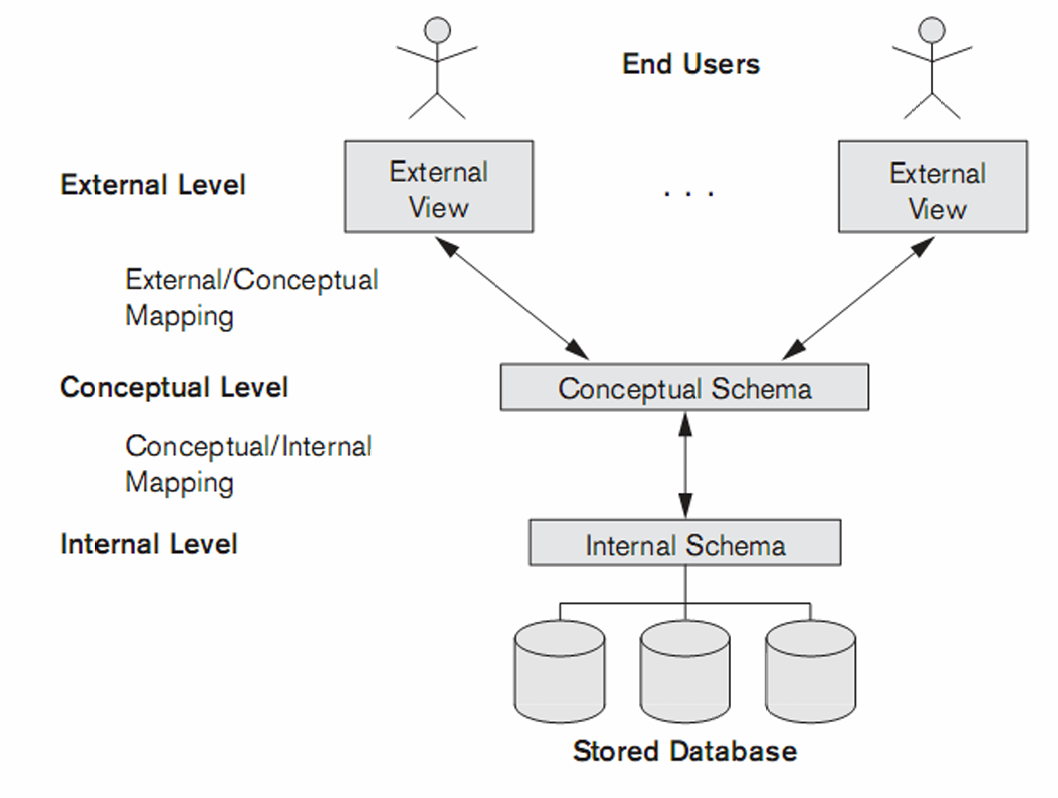
\includegraphics[width=\textwidth]{Images/ThreeSchema.png}
	\vspace{0.25cm}
	\caption{Sơ đồ biểu diễn cấu trúc 3 lớp Schema}
	\hspace*{0.5cm} Kiến trúc 3 lớp Schema bao gồm 3 thành phần là 3 lớp schema.
	\begin{enumerate}
		\item \textbf{Schema trong} mô tả cấu trúc lưu trữ vật lý của cơ sở dữ liệu
		\item \textbf{Schema luận lý} là mô tả mức độ cao của toàn bộ cơ sở dữ liệu
		\item \textbf{Schema ngoài} mô tả góc nhìn vào cơ sở dữ liệu của các nhóm người dùng khác nhau 
	\end{enumerate}
	\hspace*{0.5cm} Độc lập dữ liệu là khả năng thay đổi lược đồ ở một cấp độ của hệ thống cơ sở dữ liệu mà không cần phải thay đổi lược đồ ở cấp độ cao hơn tiếp theo.
	\begin{itemize}
		\item Độc lập dữ liệu \textbf{Luận lý}: khả năng thay đổi schema ý niệm mà không cần phải thay đổi ý niệm ngoài hoặc chương trình ứng dụng.
		\item Độc lập dữ liệu \textbf{Vật lý}: khả năng thay đổi schema trong mà không cần phải thay đổi schema ý niệm.
	\end{itemize}
\end{figure}
\subsubsection{Thiết kế Cơ sở dữ liệu}
\hspace*{0.5cm} Thiết kế Cơ sở dữ liệu là hoạt động thiết kế các cấu trúc logic và vật lý của một hoặc nhiều cơ sở dữ liệu để đáp ứng nhu cầu thông tin của người dùng trong một tổ chức cho một tập hợp các ứng dụng được xác định. Hoạt động thiết kế cơ sở dữ liệu tổng thể phải trải qua một quy trình chung có hệ thống được gọi là phương pháp thiết kế, cho dù cơ sở dữ liệu mục tiêu được quản lý bởi Hệ quản trị Cơ sở dữ liệu quan hệ hay Hệ quản trị cơ sở dữ liệu hướng đối tượng,... Kết quả của quá trình là một lược đồ cơ sở dữ liệu được định nghĩa cố định và khó có thể sửa sau khi cơ sở dữ liệu được hiện thực.\\
\hspace*{0.5cm} Mục tiêu cần đạt được trong việc thiết kế cơ sở dữ liệu tập trung chủ yếu vào việc đáp ứng các yêu cầu về nội dung thông tin của người dùng và ứng dụng được chỉ định. Cung cấp cấu trúc thông tin tự nhiên và dễ hiểu. Cũng như hỗ trợ các yêu cầu xử lý và bất kỳ mục tiêu hiệu suất nào, chẳng hạn như thời gian phản hồi, thời gian xử lý và không gian lưu trữ.\\
\begin{figure}[H]
	\centering
	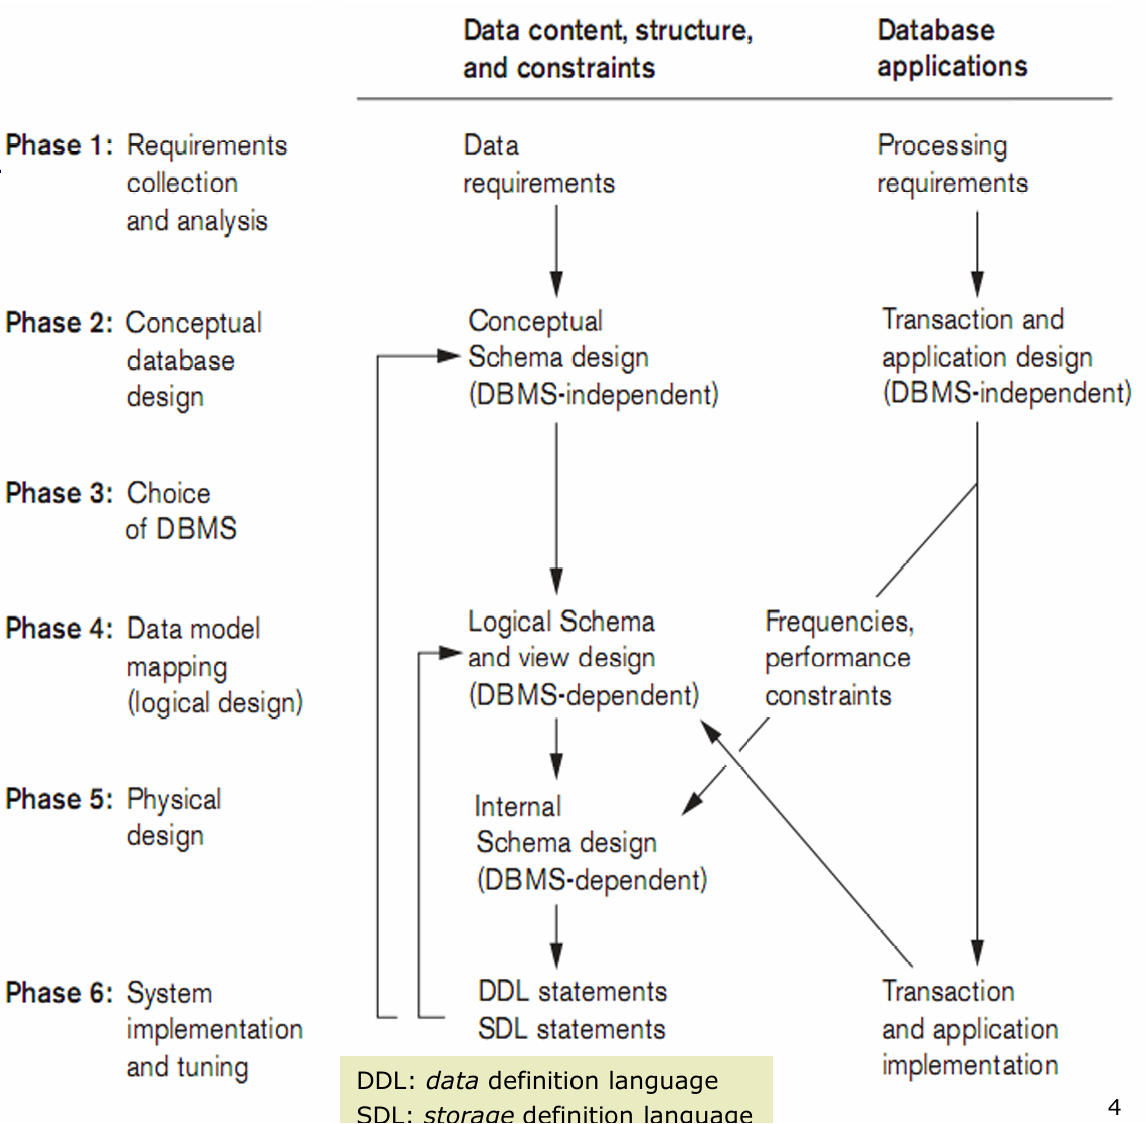
\includegraphics[width=\textwidth]{Images/DBDesign.png}
	\vspace{0.5cm}
	\caption{Quy trình thiết kế cơ sở dữ liệu}
\end{figure}
\hspace*{0.5cm} Việc thiết kế cơ sở dữ liệu trải qua 6 giai đoạn chính:
\begin{itemize}
	\item \textbf{Giai đoạn 1: Thu thập và phân tích yêu cầu}\\
	\hspace*{0.5cm} Ở bước này, người thiết kế sẽ thu thập và phân tích yêu cầu từ người dùng và ứng dụng sẽ tương tác với hệ thống cơ sở dữ liệu. Những yêu cầu này có thể được thu thập theo nhiều cách khác nhau. Trước hết cần phải xác định Lĩnh vực hoạt động chính của ứng dụng, cũng như nhóm người dùng sẽ sử dụng cơ sở dữ liệu hoặc công việc sẽ ảnh hưởng đến cơ sở dữ liệu. Tìm hiểu về tài liệu của ứng dụng sử dụng, tìm hiểm về môi trường thực thi và các kế hoạch sử dụng dữ liệu và xử lý thành thông tin, bao gồm loại giao dịch, tần suất, các yếu tố địa lý, input và output của giao dịch. Ngoài ra cần thu thập các ý kiến của người dùng về nhu cầu sử dụng, vì ưu tiên về nhu cầu của người dùng vẫn là trên hết. Quá trình này mất nhiều thời gian nhưng đóng vai trò rất quan trọng đối với sự thành công của cơ sở dữ liệu. Người thiết kế phải cố gắng xác định và phân tích kỳ vọng của người dùng và mục đích sử dụng của cơ sở dữ liệu một cách chi tiết nhất có thể để đạt được hệ cơ sở dữ liệu hiệu quả, đạt yêu cầu và giá trị mang lại cao.
	\item \textbf{Giai đoạn 2: Thiết kế cơ sở dữ liệu luận lý}\\
	\hspace*{0.5cm} Giai đoạn được chia làm 2 công việc con. Đầu tiên là thiết kế Schema Ý niệm. Mục tiêu cần đạt của công việc này là hiểu được đầy đủ về cấu trúc cơ sở dữ liệu, ngữ ngữa, mối quan hệ tương hỗ và ràng buộc. Người thiết kế cần xác định rõ được kiểu thực thể, kiểu quan hệ, thuộc tính, thuộc tính chính, số lượng và ràng buộc tham gia vào các mối quan hệ, kiểu thực thể yếu, phân cấp chuyên môn hoá/tổng quát hoá,… Người thiết kế có thể lựa chọn các cách tiếp cận yêu cầu của các ngôi để thiết kế mô hình ý niệm. Người thiết kế  có thể tổng hợp các yêu cầu lại thành một thể, rồi thiết kế ý niệm dựa trên những yêu cầu đã kết hợp đó. Hoặc cũng có thể thiết kế ý niệm cho từng nhóm yêu cầu của người dùng khác nhau, rồi tổng hợp các mô hình lại trước khi thực hiện thiết kế luận lý. Cách tiếp cận khác nhau cũng ảnh hưởng đến việc xây dựng external schema cho từng người dùng khác nhau.\\
	\hspace*{0.5cm} Một công việc trong giai đoạn này người thiết kế cần lưu tâm, đó là thiết kế giao dịch (Transaction Design), Thiết kế giao dịch bao gồm thiết kế các đặc điểm của các giao dịch (hoặc ứng dụng) cơ sở dữ liệu đã biết độc lập với DBMS để đảm bảo rằng lược đồ cơ sở dữ liệu sẽ bao gồm tất cả thông tin mà các giao dịch này yêu cầu. Xác định đầu vào/đầu ra và hành vi chức năng của giao dịch. Nhóm các giao dịch thành ba loại: giao dịch truy xuất, giao dịch cập nhật (gồm thêm dữ liệu, xoá dữ liệu và cập nhật dữ liệu), giao dịch hỗn hợp.
	\item \textbf{Giai đoạn 3: Lựa chọn Hệ quản trị cơ sở dữ liệu}\\
	\hspace*{0.5cm} Ở giai đoạn này, người thiết kế cần lựa chọn Hệ quản trị cơ sở dữ liệu phù hợp với nhu cầu của người dùng, cũng đáp ứng với điều kiện của hệ thống hiện có. Một số tác nhân có thể ảnh hưởng đến việc lựa chọn Hệ quản trị. Nó có thể là các tác nhân về kỹ thuật như tính phù hợp và loại DBMS cho tác vụ cần làm; Cấu trúc lưu trữ và đường dẫn truy cập, giao diện người dùng và lập trình viên, ngôn ngữ truy vấn cấp cao, các công cụ phát triển, tuỳ chọn kiến trúc,… được DBMS hỗ trợ; Tính di động của DBMS giữa các loại phần cứng khác nhau. Cũng có thể là các tác nhân phi kỹ thuật như chi phí mua phần mềm, chi phí bảo trì, chi phí mua phần cứng, chi phí tạo và chuyển đổi cơ sở dữ liệu, chi phí nhân sự, chi phí đào tạo, chi phí vận hành cũng như tính khả dụng của dịch vụ nhà cung cấp
	\item \textbf{Giai đoạn 4: Mapping Mô hình dữ liệu (Thiết kế cơ sở dữ liệu luận lý)}\\
	\hspace{0.5cm} Giai đoạn này các người thiết kế sẽ tạo schema ý niệm và các schema ngoài trong mô hình được hỗ trợ bởi Hệ quản trị cơ sở dữ liệu theo kiến trúc 3 schema.
	Kết quả của giai đoạn này sẽ là các câu lệnh định nghĩa dữ liệu (Data Definition Language) bằng ngôn ngữ của Hệ quản trị cơ sở dữ liệu đã chọn, chỉ định lược đồ cấp khái niệm và cấp bên ngoài của hệ thống cơ sở dữ liệu.
	\item \textbf{Giai đoạn 5: Thiết kế cơ sở dữ liệu vật lý}\\
	\hspace*{0.5cm} Giới hạn trong việc lựa chọn các cấu trúc phù hợp nhất cho
	các tệp cơ sở dữ liệu từ các tùy chọn do DBMS đó cung cấp.
	Chọn các cấu trúc lưu trữ cụ thể và đường dẫn truy cập cho
	các tệp cơ sở dữ liệu, việc lựa chọn dựa trên các yêu cầu nhất định, như thời gian phản hồi, không gian lưu trữ hiệu dụng cũng như khối lượng giao dịch. Ước tính kích thước bản ghi và số lượng bản ghi trong mỗi tệp cơ sở dữ liệu.
	Người thiết kế cần ước tính các mẫu cập nhật và truy xuất cho tệp tích lũy từ tất cả các giao dịch, cũng như ước tính sự phát triển của tệp, theo kích thước bản ghi do các thuộc tính mới hoặc theo số lượng bản ghi.
	\item \textbf{Giai đoạn 6: Hiện thực và tinh chỉnh Hệ cơ sở dữ liệu}\\
	\hspace*{0.5cm} Ở giai đoạn này, người thiết kế thực hiện các công việc như tạo các Schema cơ sở dữ liệu và các tệp tin cơ sở dữ liệu (trống); Định dạng lại dữ liệu để tải vào cơ sở dữ liệu mới nếu cần; Tải hoặc thêm dữ liệu vào bảng (nếu cần); Hiện thực các giao dịch cơ sở dữ liệu tham chiếu đến các thông số kỹ thuật ý niệm của giao dịch, sau đó viết và kiểm tra mã chương trình bằng các lệnh thuộc ngôn ngữ xử lý dữ liệu (Data Manipulation Language) nhúng. Việc điều chỉnh cơ sở dữ liệu vẫn tiếp tục miễn là cơ sở dữ liệu vẫn tồn tại, miễn là các vấn đề về hiệu suất vẫn được phát hiện và trong khi các yêu cầu vẫn thay đổi.
	
\end{itemize}
\subsection{Ngôn ngữ truy vấn SQL}
\subsubsection{SQL là gì?}
\hspace*{0.5cm} SQL được viết tắt từ Structured Query Language, là một ngôn ngữ lập trình phục vụ việc lưu trữ và xử lý thông tin trong cơ sở dữ liệu quan hệ. Cơ sở dữ liệu quan hệ lưu trữ thông tin dưới dạng bảng có các hàng và cột đại diện cho những thuộc tính dữ liệu và nhiều mối quan hệ khác nhau giữa các giá trị dữ liệu. Bạn có thể sử dụng các câu lệnh SQL để lưu trữ, cập nhật, loại bỏ, tìm kiếm và truy xuất thông tin từ cơ sở dữ liệu. Bạn cũng có thể sử dụng SQL để duy trì và tối ưu hóa hiệu suất cơ sở dữ liệu.\\
\hspace*{0.5cm} Ngôn ngữ truy vấn có cấu trúc (SQL) là một ngôn ngữ truy vấn phổ biến thường được sử dụng trong tất cả các loại ứng dụng. Các nhà phân tích và phát triển dữ liệu tìm hiểu và sử dụng SQL do ngôn ngữ này tích hợp hiệu quả với nhiều ngôn ngữ lập trình khác nhau. Theo ANSI (American National Standards Institute - Viện Tiêu chuẩn Quốc gia Hoa Kỳ), SQL là ngôn ngữ tiêu chuẩn cho các hệ thống quản lý cơ sở dữ liệu quan hệ.
\subsubsection{SQL hoạt động như thế nào?}
\hspace*{0.5cm} Việc triển khai ngôn ngữ truy vấn có cấu trúc (SQL) liên quan đến một máy chủ xử lý truy vấn cơ sở dữ liệu và trả về kết quả. Quá trình SQL đi qua một số thành phần phần mềm sau:\\
\hspace*{0.5cm}\textbf{Trình phân tích cú pháp}\\
\hspace*{0.5cm}Trình phân tích cú pháp bắt đầu bằng cách token hóa hoặc thay thế một số từ trong câu lệnh SQL bằng các ký hiệu đặc biệt. Sau đó, nó sẽ kiểm tra câu lệnh để tìm kiếm những yếu tố sau:
\begin{itemize}
	\item Tính đúng đắn: Trình phân tích cú pháp xác minh rằng câu lệnh SQL tuân theo ngữ nghĩa SQL, hay các quy tắc, đảm bảo tính đúng đắn của câu lệnh truy vấn. Ví dụ: trình phân tích cú pháp kiểm tra xem lệnh SQL có kết thúc bằng dấu chấm phẩy hay không. Nếu thiếu dấu chấm phẩy, trình phân tích cú pháp sẽ trả về lỗi.
	\item Quyền hạn: Trình phân tích cú pháp cũng xác thực rằng người dùng đang chạy truy vấn có quyền cần thiết để thao tác với dữ liệu tương ứng. Ví dụ: chỉ người dùng quản trị mới có quyền xóa dữ liệu.
\end{itemize}

% \hspace*{0.5cm}Tính đúng đắn\\
% \hspace*{0.5cm}Trình phân tích cú pháp xác minh rằng câu lệnh SQL tuân theo ngữ nghĩa SQL, hay các quy tắc, đảm bảo tính đúng đắn của câu lệnh truy vấn. Ví dụ: trình phân tích cú pháp kiểm tra xem lệnh SQL có kết thúc bằng dấu chấm phẩy hay không. Nếu thiếu dấu chấm phẩy, trình phân tích cú pháp sẽ trả về lỗi.\\

% \hspace*{0.5cm}Quyền hạn\\
% \hspace*{0.5cm}Trình phân tích cú pháp cũng xác thực rằng người dùng đang chạy truy vấn có quyền cần thiết để thao tác với dữ liệu tương ứng. Ví dụ: chỉ người dùng quản trị mới có quyền xóa dữ liệu.\\
\hspace*{0.5cm}\textbf{Công cụ quan hệ}\\
\hspace*{0.5cm}Công cụ quan hệ, hay bộ xử lý truy vấn, tạo kế hoạch truy xuất, ghi hoặc cập nhật dữ liệu tương ứng theo cách hiệu quả nhất. Ví dụ: công cụ này kiểm tra các truy vấn tương tự, sử dụng lại các phương pháp thao tác dữ liệu trước đó hoặc tạo một phương pháp mới. Công cụ quan hệ viết kế hoạch trong mã byte, một dạng biểu diễn trung cấp của câu lệnh SQL. Cơ sở dữ liệu quan hệ sử dụng mã byte để thực hiện tìm kiếm và điều chỉnh cơ sở dữ liệu một cách hiệu quả.\\
\hspace*{0.5cm}\textbf{Công cụ lưu trữ}\\
\hspace*{0.5cm}Công cụ lưu trữ, hoặc công cụ cơ sở dữ liệu, là thành phần phần mềm xử lý mã byte và chạy câu lệnh SQL dự định. Công cụ này đọc và lưu trữ dữ liệu trong các tệp cơ sở dữ liệu trên ổ đĩa lưu trữ vật lý. Sau khi hoàn tất, công cụ lưu trữ trả về kết quả cho ứng dụng yêu cầu.
\subsubsection{Các ngôn ngữ truy vấn dữ liệu SQL}
\hspace*{0.5cm}Lệnh ngôn ngữ truy vấn có cấu trúc (SQL) là những từ khóa hoặc câu lệnh SQL cụ thể được các nhà phát triển sử dụng để thao tác với dữ liệu được lưu trữ trong cơ sở dữ liệu quan hệ. Bạn có thể phân loại các lệnh SQL như sau:\\
\hspace*{0.5cm}\textbf{Ngôn ngữ định nghĩa dữ liệu}\\
\hspace*{0.5cm}Ngôn ngữ định nghĩa dữ liệu (DDL) là các lệnh SQL thiết kế cấu trúc cơ sở dữ liệu. Các kỹ sư cơ sở dữ liệu sử dụng DDL để tạo và điều chỉnh các đối tượng cơ sở dữ liệu dựa trên các yêu cầu nghiệp vụ. Ví dụ: kỹ sư cơ sở dữ liệu sử dụng lệnh CREATE để tạo các đối tượng cơ sở dữ liệu như bảng, chế độ xem và chỉ mục.\\
\hspace*{0.5cm}\textbf{Ngôn ngữ truy vấn dữ liệu}\\
\hspace*{0.5cm}Ngôn ngữ truy vấn dữ liệu (DQL) bao gồm các lệnh hướng dẫn để truy xuất dữ liệu được lưu trữ trong cơ sở dữ liệu quan hệ. Các ứng dụng phần mềm sử dụng lệnh SELECT để lọc và trả về kết quả cụ thể từ một bảng SQL.\\
\hspace*{0.5cm}\textbf{Ngôn ngữ thao tác dữ liệu}\\
\hspace*{0.5cm}Các câu lệnh ngôn ngữ thao tác dữ liệu (DML) viết thông tin mới hoặc điều chỉnh các bản ghi hiện có trong cơ sở dữ liệu quan hệ. Ví dụ: một ứng dụng sử dụng lệnh INSERT để lưu trữ một bản ghi mới trong cơ sở dữ liệu.\\
\hspace*{0.5cm}\textbf{Ngôn ngữ kiểm soát dữ liệu}\\
\hspace*{0.5cm}Quản trị viên cơ sở dữ liệu sử dụng ngôn ngữ kiểm soát dữ liệu (DCL) để quản lý hoặc cấp quyền truy cập cơ sở dữ liệu cho người dùng khác. Ví dụ: họ có thể sử dụng lệnh GRANT để cho phép các ứng dụng nhất định thao tác với một hoặc nhiều bảng.\\
\hspace*{0.5cm}\textbf{Ngôn ngữ kiểm soát giao dịch}\\
\hspace*{0.5cm}Công cụ quan hệ sử dụng ngôn ngữ kiểm soát giao dịch (TCL) để tự động thực hiện các thay đổi đối với cơ sở dữ liệu. Ví dụ: cơ sở dữ liệu sử dụng lệnh ROLLBACK để hoàn tác một giao dịch bị lỗi.
\begin{figure}[H]
	\centering
	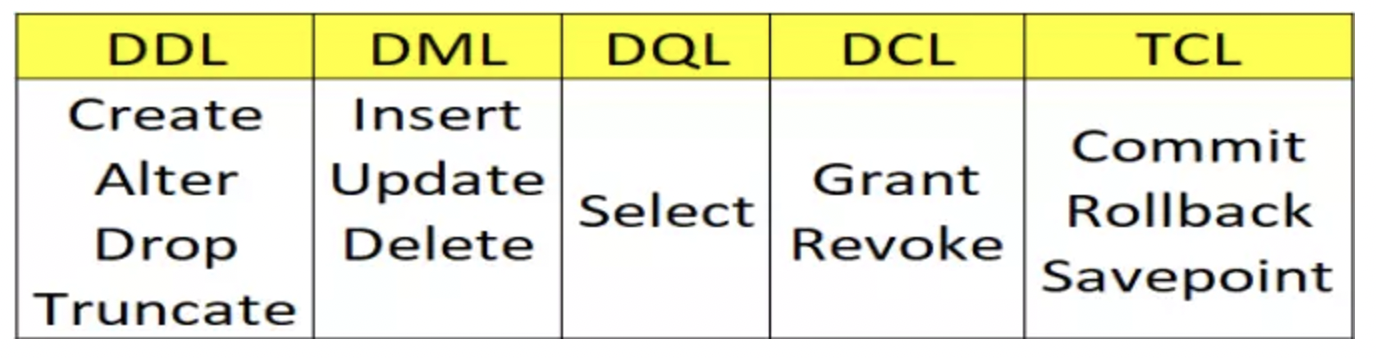
\includegraphics[width=\textwidth]{Images/lệnh SQL.png}
	\vspace{0.5cm}
	\caption{Các câu lệnh SQL cơ bản}
\end{figure}
\subsection{SQLite}
\subsubsection{SQLite là gì?}
\hspace*{.5cm}SQLite là hệ quản trị cơ sở dữ liệu (DBMS) quan hệ tương tự như Mysql,  ... Đặc điểm nổi bật của SQLite so với các DBMS khác là gọn, nhẹ, đơn giản, đặt biệt không cần mô hình Server - Client, không cần cài đặt, cấu hình hay khởi động nên không có khái niệm User, Password hay quyền hạn trong SQLite Database. Dữ liệu cũng được lưu ở một file duy nhất.\\
\hspace*{.5cm} SQLite thường không được sử dụng với các hệ thống lớn nhưng với những hệ thống ở quy mô vừa và nhỏ thì SQLite không thua các DBMS khác về chức năng hay tốc độ. Vì không cần cài đặt hay cấu hình nên SQLite được sử dụng nhiều trong việc phát triển, thử nghiệm vì tránh được những rắc rối trong quá trình cài đặt.
\subsubsection{Ưu điểm}
\begin{itemize}
	\item Giao dịch trong SQLite tuân thủ theo nguyên tắc (ACID) ngay cả sau khi hệ thống treo và mất điện.
	\item SQLite không cần mô hình Client – Server để hoạt động. Các thao tác dữ liệu trên SQLite chạy nhanh hơn so với các hệ quản trị cơ sở dữ liệu theo mô hình Client – Server.
	\item SQLite không cần phải cấu hình. SQLite rất đơn giản và dễ dàng sử dụng.
	\item SQLite hỗ trợ hầu hết các tính năng của ngôn ngữ truy vấn SQL theo chuẩn SQL92.
	\item Một sở dữ liệu hoàn chỉnh được lưu trữ trong một tệp đa nền tảng duy nhất. Phù hợp với sử dụng dưới dạng định dạng tệp ứng dụng.
	\item Một sở dữ liệu hoàn chỉnh được lưu trữ trong một tệp đa nền tảng duy nhất. Phù hợp với sử dụng dưới dạng định dạng tệp ứng dụng.
	\item Đa nền tảng: Android, iOS, Linux, Mac, Solaris, Windows,.. Dễ dàng dịch chuyển sang các hệ thống khác.
	\item SQLite rất nhỏ gọn, bản đầy đủ các tính năng nhỏ hơn 500kb, và có thể nhỏ hơn nếu lược bớt một số tính năng. Với đặc tính nhỏ gọn, truy xuất dữ liệu nhanh SQLite thường được sử dụng để nhúng vào các dự án.
\end{itemize}
\subsubsection{Nhược điểm}
\begin{itemize}
	\item Một số tính năng của SQL92 không được hỗ trợ trong SQLite như ALTER DROP COLUMN, ADD CONSTRAINT, RIGHT JOIN, TRIGGER, phân quyền GRANT và REVOKE.
	\item Vì SQLite không cần cấu hình, cài đặt, không hỗ trợ GRANT và REVOKE nên việc phân quyền truy cập cơ sở dữ liệu chỉ có thể là quyền truy cập file của hệ thống.
	\item Do sử dụng cơ chế coarse-gained locking nên trong cùng một thời điểm SQLite có thể hỗ trợ nhiều người đọc dữ liệu, nhưng chỉ có 1 người có thể ghi dữ liệu.
	\item SQLite không phải là lựa chọn hoàn hảo để đáp ứng các nhu cầu xử lý trên một khối lượng dữ liệu lớn, phát sinh liên tục.
\end{itemize}
\subsection{Dependency Injection Design Pattern} 
\subsubsection{Dependency Injection là gì?}
\hspace*{0.5cm} Dependency Injection Design Pattern là một quá trình trong đó chúng ta tiêm (inject) đối tượng phụ thuộc (dependencies) của một lớp vào một lớp phụ thuộc đối tượng đó. Dependency Injection Design Pattern là mẫu thiết kế được sử dụng phổ biến nhất hiện nay để loại bỏ sự phụ thuộc giữa các đối tượng.\\
\hspace*{0.5cm} Dependency Injection (DI) là một mẫu thiết kế được sử dụng để triển khai Inversion of Control. Nó cho phép tạo các đối tượng phụ thuộc bên ngoài một lớp và cung cấp các đối tượng đó cho một lớp phụ thuộc vào nó. Mẫu thiết kế DI bao gồm 3 lớp:
\begin{itemize}
	\item Lớp Client: Lớp Client (lớp phụ thuộc) là lớp phụ thuộc vào Lớp Service. Điều đó có nghĩa là Lớp Client muốn sử dụng các Dịch vụ (Phương thức) của Lớp Service.
	\item Lớp Service: Lớp Service (phụ thuộc) là lớp cung cấp các dịch vụ thực tế cho lớp máy khách.
	\item Lớp Injector: Lớp Injector là lớp đưa đối tượng Lớp dịch vụ vào Lớp máy khách.
\end{itemize}
\begin{figure}[H]
	\centering
	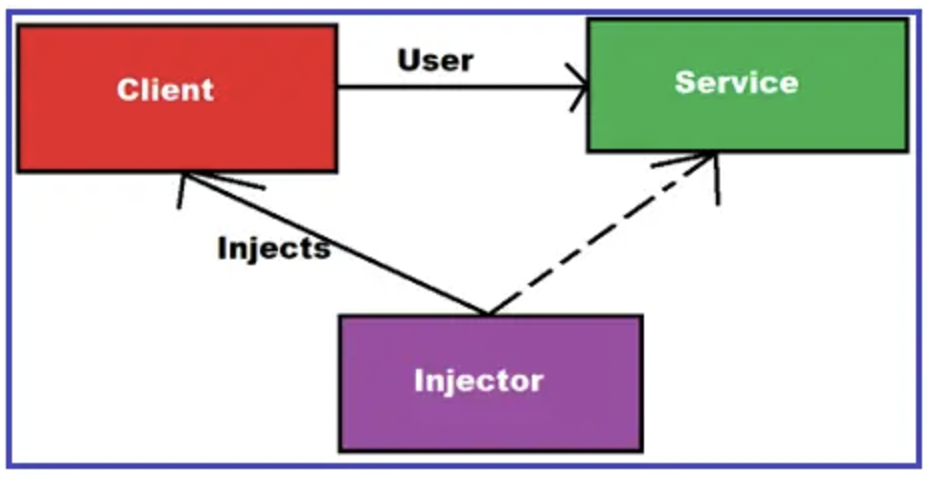
\includegraphics[width=\textwidth]{Images/DI_diagram.png}
	\vspace{0.25cm}
	\caption{Sơ đồ biểu diễn Dependency Injection}
\end{figure}
\hspace*{0.5cm} Như bạn có thể thấy, Lớp Injector tạo một đối tượng của Lớp dịch vụ và inject đối tượng đó vào Lớp Client. Sau đó, Lớp Client sử dụng Đối tượng được inject của Lớp Service để gọi các Phương thức của Lớp Service. Vì vậy, theo cách này, DI tách trách nhiệm tạo đối tượng của lớp Service ra khỏi Lớp Client. 
\subsubsection{Các loại Dependency Injection}
\hspace*{0.5cm} Lớp Injector đưa Dependency Object vào Lớp Client theo ba cách khác nhau:
\begin{itemize}
	\item Constructor injection: Các dependency (biến phụ thuộc) được cung cấp thông qua constructor (hàm tạo lớp).
	\item Setter injection: Các dependency sẽ được truyền vào 1 class thông qua các setter method (hàm setter).
	\item Interface injection: Dependency sẽ cung cấp một Interface, trong đó có chứa hàm có tên là Inject. Các client phải triển khai một Interface mà có một setter method dành cho việc nhận dependency và truyền nó vào class thông qua việc gọi hàm Inject của Interface đó.
\end{itemize}
\hspace*{0.5cm} Trong ba kiểu Inject thì phương thức Constructor injection là phổ biến nhất vì tính linh hoạt, mềm dẻo và dễ xây dựng thư viện DI.
\subsubsection{Ưu và khuyết điểm}
\hspace*{0.5cm} \textbf{Ưu điểm}
\begin{itemize}
	\item Giảm sự kết dính giữa các module.
	\item Code dễ bảo trì, dễ thay thế module.
	\item Rất dễ test và viết Unit Test.
	\item Dễ dàng thấy quan hệ giữa các module (Vì các dependency đều được inject vào constructor).
\end{itemize}
\hspace*{0.5cm} \textbf{Khuyết điểm}
\begin{itemize}
	\item Các developer mới sẽ gặp khó khăn khi học về DI.
	\item Sử dụng interface nên đôi khi sẽ khó debug, do không biết chính xác module nào được gọi.
	\item Các object được khởi tạo toàn bộ ngay từ đầu, có thể làm giảm performance.
	\item Làm tăng độ phức tạp của code.
\end{itemize}
\subsection{Observer Design Pattern}
\subsubsection{Giới thiệu}
\begin{itemize}
	\item Observer Pattern là một mẫu thiết kế thuộc nhóm Behavioral Pattern.
	\item Định nghĩa mối phụ thuộc một - nhiều giữa các đối tượng để khi mà một đối tượng (subject) có sự thay đổi trạng thái, tất cả các thành phần phụ thuộc của nó (observer) sẽ được thông báo và cập nhật một cách tự động.
	\item Một đối tượng có thể thông báo đến một số lượng không giới hạn các đối tượng khác.
\end{itemize}
\hspace*{0.5cm} Observer Pattern được áp dụng khi:
\begin{itemize}
	\item Sự thay đổi trạng thái ở 1 đối tượng có thể được thông báo đến các đối tượng khác mà không phải giữ chúng liên kết quá chặt chẽ.
	\item Cần mở rộng dự án với ít sự thay đổi nhất.
\end{itemize}
\subsubsection{Kiến trúc}
\begin{figure}[H]
	\centering
	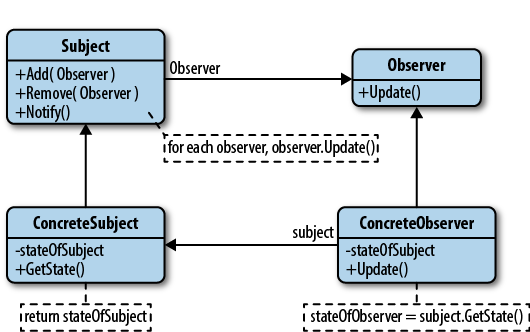
\includegraphics[width=0.75\textwidth]{Images/observer.png}
	\vspace{0.5cm}
	\caption{Kiến trúc của Observer Design Pattern}
\end{figure}
\hspace*{0.5cm} \textbf{Subject}
\begin{itemize}
	\item Biết danh sách không giới hạn các observers của nó.
	\item Cung cấp một giao diện để có thể thêm và loại bỏ observer.
\end{itemize}
\hspace*{0.5cm} \textbf{Observer}
\begin{itemize}
	\item Định nghĩa một giao diện cập nhật cho các đối tượng sẽ được subject thống báo đến khi có sự thay đổi trạng thái.
\end{itemize}
\hspace*{0.5cm} \textbf{ConcreteSubject}
\begin{itemize}
	\item Lưu trữ trạng thái danh sách các ConcreateObserver.
	\item Gửi thông báo đến các observer của nó khi có sự thay đổi trạng thái.
\end{itemize}
\hspace*{0.5cm} \textbf{ConcreteObserver}
\begin{itemize}
	\item Có thể duy trì một liên kết đến đối tượng ConcreteSubject.
	\item Lưu trữ trạng thái của subject.
	\item Thực thi việc cập nhật để giữ cho trạng thái đồng nhất với subject gửi thông báo đến.
\end{itemize}
\hspace*{0.5cm}Khi subject có sự thay đổi trạng thái, nó sẽ duyệt qua danh sách các observer của nó và gọi phương thức cập nhật trạng thái ở từng observer, có thể truyền chính nó vào phương thức để các observer có thể lấy ra trạng thái của nó và xử lý.
\begin{figure}[H]
	\centering
	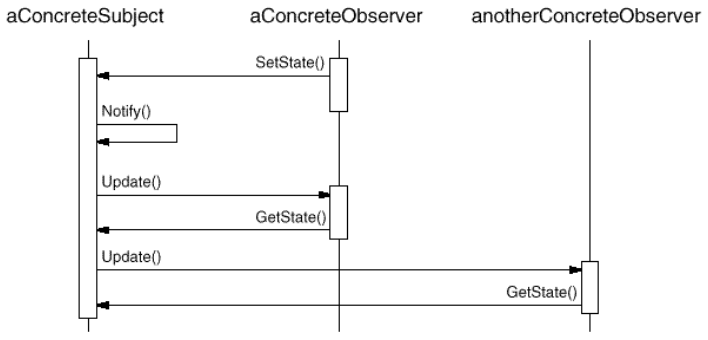
\includegraphics[width=0.75\textwidth]{Images/observer_work.png}
	\vspace{0.5cm}
	\caption{Tương tác giữa subject và các observer}
\end{figure}
\subsubsection{Ưu và nhược điểm}
\hspace*{.5cm} \textbf{Ưu điểm}
\begin{itemize}
	\item Đảm bảo nguyên tắc Open/Closed Principle (OCP): Cho phép thay đổi Subject và Observer một cách độc lập. Chúng ta có thể tái sử dụng các Subject mà không cần tái sử dụng các Observer và ngược lại. Nó cho phép thêm Observer mà không sửa đổi Subject hoặc Observer khác.
	\item Thiết lập mối quan hệ giữa các objects trong thời gian chạy.
	\item Sự thay đổi trạng thái ở 1 đối tượng có thể được thông báo đến các đối tượng khác mà không phải giữ chúng liên kết quá chặt chẽ.
	\item Không giới hạn số lượng Observer
\end{itemize}
\hspace*{.5cm} \textbf{Nhược điểm}
\begin{itemize}
	\item Unexpected update: Bởi vì các Observer không biết về sự hiện diện của nhau, nó có thể gây tốn nhiều chi phí của việc thay đổi Subject.
	\item Subscriber được thông báo theo thứ tự ngẫu nhiên.
\end{itemize}
\subsection{Unity Engine và C\#}
Trong quá trình phát triển trò chơi điện tử, mỗi một tựa game là những thực thể độc lập, được thực hiện theo những cách khác nhau và có những điểm đặc trưng riêng của tựa game đó. Tuy nhiên, việc xây dựng một tựa game từ móng thì sẽ rất tốn thời gian và công sức. Có những thành phần tổng quát, cơ bản có thể được dùng đi dùng lại cho nhiều trò chơi khác nhau. Ví dụ cách vật lý và trọng lực tác động lên các vật thể đều giống nhau. Hoặc cách phát âm thanh trong trò chơi cũng có thể tổng quát hóa được. Một ví dụ nữa là việc phát hiện và xử lý va chạm của đa số trò chơi cũng phát triển dựa trên cùng một nền tảng lý thuyết. Do đó, người ta nhận ra rằng có thể tạo ra một bộ khung (framework) hay một hệ thống (infrastructure) làm nền tảng để việc phát triển trò chơi trở nên thuận tiện và hiệu quả hơn. Bộ khung hoặc hệ thống này được gọi là game engine.\footnote{Alan Thorn, \textit{Game Engine Design and Implementation 1st Editio}n, tr.6}\\

Unity là một trong những engine phát triển game phổ biến nhất hiện nay. Unity cung cấp cho người dùng một nền tảng để tạo ra các trò chơi, ứng dụng 2D và 3D một cách thuận tiện và có hệ thống. Ưu điểm của việc sử dụng engine đó là engine sẽ hỗ trợ sẵn những cơ chế cốt lõi của một trò chơi điện tử bao gồm render đồ họa 2D và 3D, tính toán vật lý và va chạm, âm thanh, animation ... Lý do nhóm nghiên cứu chọn sử dụng Unity engine bởi vì Engine này phổ biến, dễ tiếp cận và cực kỳ phù hợp với dự án game vừa và nhỏ. Một điểm cộng nữa là cộng đồng sử dụng Unity Engine rất lớn. Điều này khiến việc vừa làm vừa học hỏi trở nên dễ dàng hơn nhờ nguồn tài liệu và hướng dẫn vô cùng phong phú.\\

Ngôn ngữ lập trình được sử dụng cùng với Unity là C\#. C\# là một ngôn ngữ lập trình thuần hướng đối tượng, rất phù hợp với phát triển hệ thống component-based. Điểm mạnh của C\# là cú pháp tuy đơn giản nhưng rất chặt chẽ và linh hoạt, giúp cho nhà phát triển dễ dàng hiện thực những ý tưởng sáng tạo của mình.\\